\chapter{Discussion}
\label{Chap5}
\section{Powder ageing}
\subsection{Grain size and distribution}

Two trends were identified in section \ref{RGSAD}: there was a clear diminution of the average particle size $D_a$ and a narrowing of the distribution as functions of the number or recycling iterations. Only one sampling did not concur with these observations. This can be easily explained: the powder in question was sampled just after fresh powder was added to the recycled one. Its size distribution was thus shifted back towards a fresher distribution. \\
%modified in a way that is opposed to what recycling causes. \\

Particle sizes going up to $\simeq 134$ [$\mu m$] were measured in the powder samples even though they were sieved with a 75 [$\mu m$] mesh size. The most reasonable justification is that particles agglomeration took place between the siftings and the sizes measurements. Ultrasonic treatments gave the opportunity to confirm that a non-negligible part of the AlSi10Mg powder indeed agglomerated. The maximal measured particle size after exposure to ultrasounds was $\simeq 84$ $[mu m]$. This is rather close to the sieving mesh size but still bigger. The gap between the two could be due to lack of resolution or to residual aggregates.\\

The agglomeration phenomena could explain the diminution of the average particle size with the recycling iterations, according to Maamoud et al. (2018) \cite{Maamoud18}: the large particles that agglomerated since the last sieving could not go through the mesh. Only smaller particles were thus recycled, lowering the average size. Another cause could be the projection of very fine spatters out of the melt pool during the process. These spatters could fall in the unmelted powder and be recycled with the it. Unfortunately, no source could be found literature to support or refute this hypothesis.\\
%. Small particles could also have been preferentially scattered during the SLM process. They would have thus been retrieved in bigger proportion right after

 It seems reasonable to assume that the agglomerates could have led to the emergence of defects in the parts due to powder bed inhomogeneity. This could, at least partly, explain the scatter of relative densities for samples from a same batch. %It may also be a reason behind the remarkably poor properties of sample "8a" (see section \ref{RReprod}).\\
\subsection{Composition}

ICP spectrometry was used in order to estimate the impact of repeated recycling on the evolution of the chemical elements mass fractions. A few observations were made. The prior addition of fresh powder of February sample increased the mass fractions of iron, magnesium, and potentially silicon. It seems that there is a systematic diminution of the alloying elements with the reuse of the powder. Unfortunately, this cannot be attested due to the large error bars.\\

The change of composition induced by SLM was also investigated for two samples. It was concluded that approximately 4\% of the magnesium was lost during the process. The preferential loss of magnesium for a heated aluminium-based alloy is well known \parencite{HIDVEGI197739}. It is due to the lower vapour pressure of the element. %A slight loss of silicon also seemed to have taken place ($\simeq 1\%$) but this cannot be certified.
\section{Density measures assessments}
\label{DDMA}

%\subsection{Hydrostatic weighing}


\subsection{Relative optical density image analysis}
\label{DRODIA}

The estimation of the relative density through RODIA can be imprecise on many aspects. First, the distribution of porosities is inhomogeneous on the analysed surface. Multiple pictures must thus be taken systematically and arbitrarily for each specimen to constitute a representative sample.\\

Second, the quality of the images has a critical role. The isolation of the porosities during the thresholding requires a substantial difference of pixel intensity between the holes and the material. Since some porosities and some zones of the material can appear respectively brighter or darker than was is expected, there are risks that one isolates spots and/or not actual porosities. Additionally, the thresholding is manual and thus prone to slight human errors. \\

Most importantly, the finite resolution of the camera implies that the smallest porosities are not visible on the pictures. One can expect the density measurement through RODIA to be a biased method, due to the discretisation in pixels among other things. Results for pictures with different magnifications were compared to quantify these effects. For this purpose, a picture was taken under 5x magnification and two under 10x magnification. The former was delimited to match the visible zones on the latter (see figure \ref{fig:RODIA1}). The same two zones - named A and B - were thus analysed for different levels of resolution.\\

\begin{figure}[ht]
	\centering
	\centerline{\includegraphics[scale=0.075]{Images/RODIA1}}
	\decoRule
	\caption[5x magnification picture of specimen X200-180319-cub1 and delimitation of the zones A and B]{5x magnification picture of specimen X200-180319-cub1 and delimitation of the zones A and B}
	\label{fig:RODIA1}
\end{figure}

\begin{figure}[ht]
	\centering
	\centerline{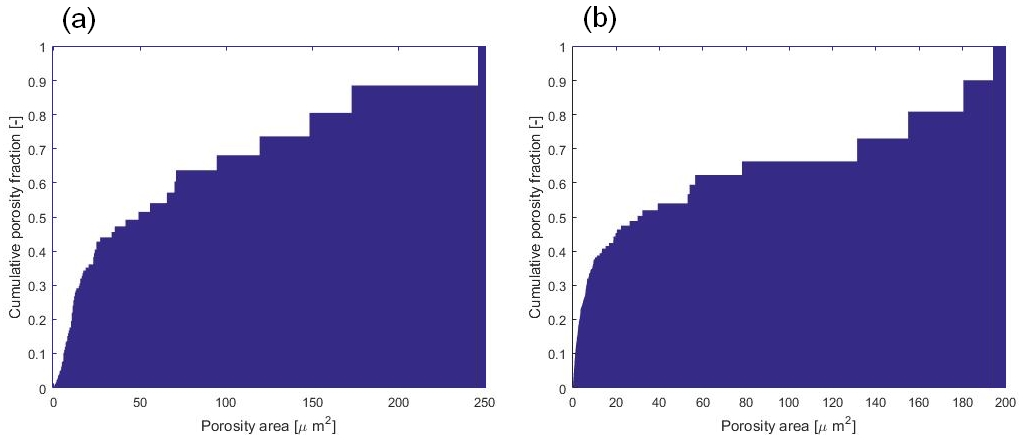
\includegraphics[scale=0.7]{Images/CumSum}}
	\decoRule
	\caption[Cumulative porosity fraction bar chart as function of the porosity area from picture of specimen X200-180319 on zone A under (a) 5x magnification (b) 10x magnification]{Cumulative porosity fraction bar chart as function of the porosity area from picture of specimen X200-180319 on zone A under (a) 5x magnification (b) 10x magnification}
	\label{fig:CumSum}
\end{figure}


The comparison of figures \ref{fig:RODIA2} (b) and (d) shows that much more small porosities are isolated if the resolution is refined. This is confirmed by the bar charts on figure \ref{fig:CumSum}. The threshold of porosity area for detection in the case of 5x magnification is 0.5625 [$\mu m^2$] whereas it is 0.14 [$\mu m^2$] for 10x magnification. This area corresponds to a pixel in each case. It is also worth noting that there is an overall tendency to overestimate the areas at lower resolution, which counterbalances slightly the low number of detected porosities. \\

\begin{figure}[ht]
	\centering
	\centerline{\includegraphics[scale=0.44]{Images/RODIA2}}
	\decoRule
	\caption[Zone A of specimen X200-180319-cub1: (a) Delimitation from original picture under 5x magnification (b) Porosities isolation from 5x magnification picture (c) Original picture under 10x magnification (d) Porosities isolation of 10x magnification picture]{Zone A of specimen X200-180319-cub1: (a) Delimitation from original picture under 5x magnification (b) Porosities isolation from 5x magnification picture (c) Original picture under 10x magnification (d) Porosities isolation of 10x magnification picture}
	\label{fig:RODIA2}
\end{figure}


The RODIA results for zones A and B are outlined in table \ref{tab:RODIASS}. It was observed that pictures with lower resolution have the tendency to lead to the overestimation of the relative density. The order of magnitude of the difference is of few hundredths of percent. The method is thus presumably positively biased. However, the observed effect is minor: this is probably due to the fact that the undetected porosities are the smallest, which influence the less the calculated density value.\\

\begin{center}
	\begin{table}[ht]
		\centerline{\begin{tabular}{|c|c|c|}
				\hline
				Zone & Magnification & Measured relative density [$\%$] \\
				\hline
				A & 5x  & 99.87\\
				A & 10x & 99.84\\
				B & 5x & 99.86\\
				B & 10x & 99.85\\
				\hline
		\end{tabular}}
		\caption[RODIA results for zones A and B of specimen X200-180317 with 5x and 10x magnification]{RODIA results for zones A and B of specimen X200-180317 with 5x and 10x magnification}
		\label{tab:RODIASS}
	\end{table}
\end{center}

Taking pictures at refined magnification could be considered to refine the precision of the method. This would, however, require to increase the number of analysed pictures to generate a sample size as representative. A picture with doubled magnification covers indeed four times less surface. The number of analyses should thus be quadrupled to take as much information into account.\\

RODIA method required to make the assumption that the volumetric porosity fraction is equal the surface one. The dependability of this affirmation will now be discussed. Let us consider a cubic cell of side length D containing a spheric porosity of diameter D in its center (see figure \ref{fig:DDD}). The volumetric porosity fraction $f_v$ is:\\

$$f_v = \frac{\frac{\pi D^3}{6}}{D^3}= \frac{\pi}{6}$$

\begin{figure}[ht]
	\centering
	\centerline{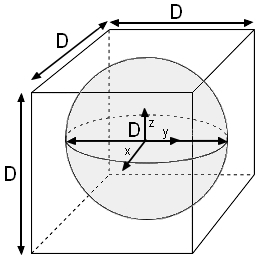
\includegraphics[scale=0.64]{Images/DDD}}
	\decoRule
	\caption[Schematic of a spheric porosity of diameter D in a cubic cell of size length D]{Schematic of a spheric porosity of diameter D in a cubic cell of size length D}
	\label{fig:DDD}
\end{figure}

However, the surface porosity fraction depends on the observed pore diameter $D_{obs}$ which varies with the z coordinate of the surface plane crossing it: $\frac{D_{obs}(z)}{2}=\sqrt{(\frac{D}{2})^2-z^2}$. If we assume that there is a statistically significant number of pores of similar size, one can make the hypothesis that - in average - the observed diameter is the mean diameter $D_{mean}$:\\

$$ \frac{D_{mean}}{2}= \frac{\int_{-\frac{D}{2}}^\frac{D}{2} D_{obs}(z) dz}{D}=\frac{\pi D}{8}$$

This hypothesis is quiet coherent for small pores but not  for the largest: in most cases, a very small number of pores is significantly bigger than the others. If we still assume it to be true, the surface porosity fraction $f_s$ can be computed as follows:

$$f_s=\frac{\frac{\pi D_{mean}^2}{4}}{D^2}=\frac{\pi^3}{16 \cdot 4} \simeq 0.9253 f_v$$

It can thus be concluded that the method to measure the relative density intrinsically has a slightly built-in positive bias. The greater the porosity is, the bigger the bias. In the working range of $\rho_{rel}$ of this work, they can go from 0.01 to 0.03 [\%]. Combining this with the bias induced by the measures imperfections, one can conclude that RODIA should be used as a mean to estimate an upper limit for the relative densities.

\subsection{Measures comparison}
Some samples' densities were also measured through hydrostatic weighing (both with and without preliminary polishing). Multiple techniques were performed on the same few specimens in order to draw a comparison of the results and reach a deeper understanding of the methods reliability. The results are gathered on figures \ref{fig:7comp} and \ref{fig:2comp}.\\

\begin{figure}[ht]
	\centering
	\centerline{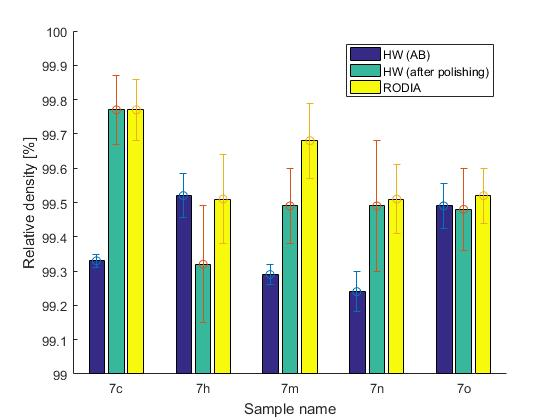
\includegraphics[scale=0.64]{Images/7comp}}
	\decoRule
	\caption[Bar chart of the density measurements with the HW (AB and after polishing) and RODIA methods for samples of batch X200-180109]{Bar charts of the density measurements with the HW (AB and after polishing) and RODIA methods for samples of batch X200-180109}
	\label{fig:7comp}
\end{figure}

\begin{figure}[ht]
	\centering
	\centerline{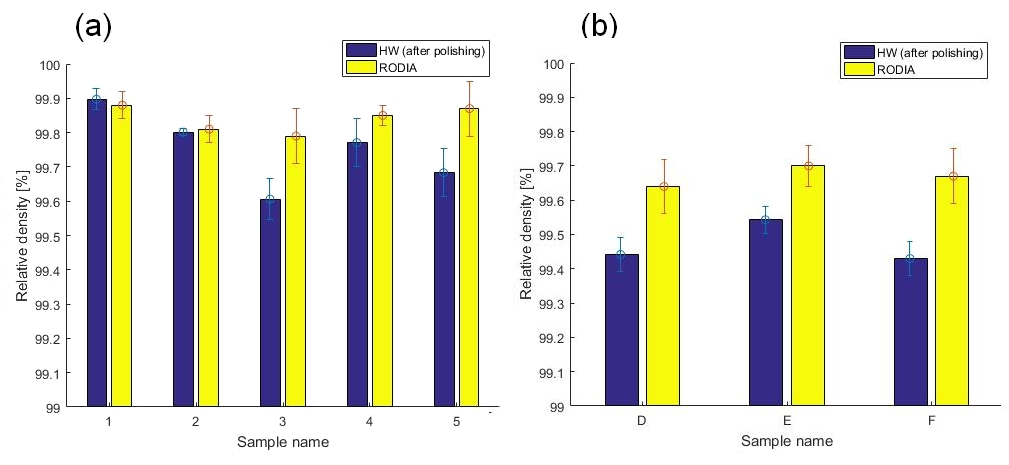
\includegraphics[scale=0.64]{Images/2comp}}
	\decoRule
	\caption[Bar charts of the density measurements with the HW (after polishing) and RODIA methods for samples of (a) batch X200-180319 (b) batch X200-180417]{Bar charts of the density measurements with the HW (after polishing) and RODIA methods for samples of (a) batch X200-180319 (b) batch X200-180417}
	\label{fig:2comp}
\end{figure}

As-built hydro measurements on figure \ref{fig:7comp} demonstrated high variability relatively to the other measures. Over the five tested samples, two exhibited similar relative densities for all techniques. However, three had $\rho_{a,rel}$ significantly below the values obtained with the other methods. In particular, the gap for sample "7c" was 0.44 [\%]. The fact that the CI do not intersect with the others' suggest that AB HW method was negatively biased in those cases. The most plausible explanation is that air was trapped in the surface roughness, which distorted the results (by overestimating the closed porosities volume. This would not be surprising as SLM produced parts usually have bad surface finish.\\ %to observe potential inhomogeneous distributions of the closed porosities in the specimens.

The two other methods were more promising. Relative densities obtained with RODIA method are generally close to the ones of HW after polishing (see figures \ref{fig:7comp} and \ref{fig:2comp}). In average, the absolute difference between the two is 0.16 [\%] (0.24 [\%] at most).  When the difference is greater than 0.02 [\%], the RODIA method always give greater density values. In addition, the CI do not always intersect. This can be attributed to the RODIA positive bias, and potentially to a negative bias for HW - that would still not be fully erased through polishing. Ultimately, given the opposite bias and the proximity of the relative density values for both methods, one could consider the two to be bounds between which lies the actual $\rho_{rel}$.\\

\section{Density and hardness study}

\subsection{Parameters optimisation}
Optimisations of the relative density and hardness were both achieved with the parameters set ($P=0.75 P_{max}=205 [W]$ , $v_s=1200 [\frac{mm}{s}]$). This pair of parameters lie in the process window suggested in section \ref{pp}.
Kempen et al. found optimal parameters values (maximising density) that are not far to the ones of this work (see table \ref{tab:compKemp}) \parencite{Kempen110817}. The energy density was however significantly bigger in this work, especially since the laser was more focused (which is not taken into account for the approximate computation). $E_d$ is rather close to a value minimising porosity obtained by Read et al. (65 $[\frac{J}{mm^3}]$) \parencite{Read150417}. Both cited sources used a chessboard scanning strategy, with islands size of around  5 x 5 [$mm^2$]. \\

\begin{center}
	\begin{table}[ht]
		\centerline{\begin{tabular}{|c|c|c|c|c|c|c|}
				\hline
				Source & h [$\mu m$] & t [$\mu m$]  & $\phi_{99\%} [\mu m]$& P $[W]$ &$v_s [\frac{mm}{sec}]$ & $E_d [\frac{J}{mm^3}]$ \\
				\hline
				This work & 100  & 30 & 75 & 205 & 1200 & 57\\
				\parencite{Kempen110817} & 105 & 30 & 150 & 200 & 1400  & 45 \\
				\parencite{Read150417} & 75 & 30  & 150 & 200 & 1350 & 65 \\				
				\hline
		\end{tabular}}
		\caption[Optimised manufacturing parameters comparison with literature sources]{Optimised manufacturing parameters comparison with literature sources}
		\label{tab:compKemp}
	\end{table}
\end{center}

A relative density of 99.9 [\%] was reached, which is superior to the best values found in the literature \parencite{EOS}. It is likely that all samples manufactured with the optimised parameters had $\rho_{rel}>99.4[\%]$ according to the measurements. Results depended on the powder age and recycling (\ref{RPI}). It can be confirmed that the parameters chosen allowed for a right energy input and a correct melt pools overlapping. \\

The hardness was significantly bigger than what is typically expected - approximately 10 [HV] more (see section \ref{MMABMP}). This could indicate that the microstructure was finer than was is typically obtained or that the material had a more pronounced work hardening ability. At first glance, nothing would justify this. A more credible justification is measurement-related: first, the obtained $H_V$ value depends significantly on the load and on the test's time length. A study showed that the Vickers hardness of aluminium 17-ST alloy - which has a comparable $H_v$ as AlSi10Mg - can range from 130.8 to 143.0 depending on the testing conditions, as shown in table \ref{tab:Vickm} \parencite{Arbtin}. This alone could explain the high hardnesses measured in this work as the load and the time length were both small (respectively 10 [kg] and 10 [sec]).\\

In addition, the indenting machine used necessitates to take manual measurements. Given the high sensitivity of the hardness as a function of the lengths measured, the slightest error is greatly amplified. For example, a length error of 5[$\mu m$], which is the achievable accuracy, induces an error of 4 [HV]. Although the repeated testing greatly improves the estimation reliability (see confidence intervals in section \ref{Rparaopti}), a slight negative bias could induce a systematic overestimation of the hardness by a few [HV]. For these reasons, the hardness values obtained in this work should not be compared to the ones in literature. However, they still can be compared to each other as they were obtained through the same procedure.\\

\begin{table}[ht]
		\centering
			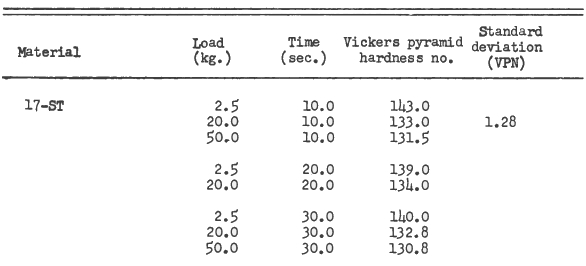
\includegraphics[scale=0.90]{Images/Vickm}
			\decoRule
		\caption[Vickers hardness results data for aluminium 17-ST alloy.]{Vickers hardness results data for aluminium 17-ST alloy (from Emil Arbtin Jr. and Glenn Murphy, 1953 \parencite{Arbtin}).}
		\label{tab:Vickm}
\end{table}

Furthermore, one should note that the optimisation of the overall density was perhaps not the most pertinent to conduct. As it will be discussed in section \ref{DMPP}, it is very likely that the tensile mechanical properties are dictated by the residual stresses and by the effects due to a second population of porosities. It could thus be interesting to perform a parametric study putting these at the forefront.\\ 

\subsection{Reproducibility}

SLM process demonstrated a satisfying reproducibility for the optimised set of parameters. However, non optimal values (P=0.75$P_{max}$,$v_s=900 [\frac{mm}{sec}]$) lead to higher variability for the hardness and the relative density. Since the energy density is bigger in that case ($76[\frac{J}{mm^3}]$), the explanation could be that the heat input was sufficient to trigger key hole instability at times, inducing porosity inside the melt pools. The phenomenon is illustrated in figure \ref{fig:KHI}. \\

\begin{figure}[ht]
	\centering
	\centerline{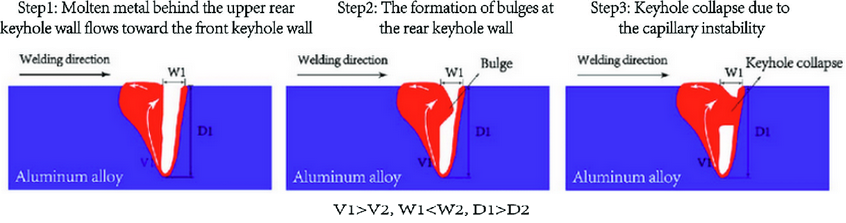
\includegraphics[scale=0.52]{Images/KHI}}
	\decoRule
	\caption[The diagram of keyhole collapse caused by the keyhole instability.]{The diagram of keyhole collapse caused by the keyhole instability (from Huang et al., 2017 \parencite{Huang2017})}
	\label{fig:KHI}
\end{figure}

Relative density tended to be bigger for the samples of parameters (P=0.75$P_{max}$,$v_s=900 [\frac{mm}{sec}]$) scanned tardily. It may be due to the longer time left to exchange heat with the nearby unsintered powder. If the first scanned samples stayed at a significantly higher temperature compared to the others, they could be more prone to exceed the threshold leading to key hole instability. They would also have a bigger hydrogen solubility, as it increases with temperature (see figure \ref{fig:Solub}) \parencite{Verhaeghe}. The apparition of porosities would thus be facilitated. \\

One sample, named X200-171024-8a, had notably low relative density. Its melt pools size distribution was compared to another specimen's (see section \ref{rs_mps}): the former was more homogeneous. Lots of porosities were present at the pools interface, which confirms that poor overlapping was achieved. The origin of this problem was not sorted out. \\


\begin{figure}[ht]
	\centering
	\centerline{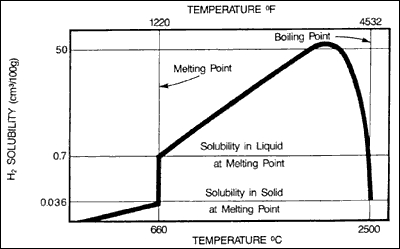
\includegraphics[scale=0.75]{Images/Solub}}
	\decoRule
	\caption[Solubility of hydrogen in aluminium.]{Solubility of hydrogen in aluminium (from Verhaeghe et al., 2003 \parencite{Verhaeghe})}
	\label{fig:Solub}
\end{figure}

The hypothesis of thermal influence do not seem to stand for the specimens made with the optimised parameters. The energy density is 33\% inferior, so the temperature must have reached lower values. No trend could thus be observed. The most determinant variables in terms of density and hardness seem to be the composition and the grain size distribution of the powder. A superior relative density was obtained after fresh powder was added to the recycled one (see section \ref{RPI}). However, an additional recycling iteration of the same powder caused a sensible decrease of $\rho_{rel}$. It dovetailed with a diminution of the alloying elements mass fractions. It is possible that both trends were correlated. Another possibility is that the contamination with moisture exceeded a critical value. The latter cannot be measured with ICP so this could not be verified.

\section{Mechanical properties}
\label{DMPP}
The average tensile properties measures for AB specimens fell a bit short of the expectations. While $\sigma_y$ was elavated compared to the standards, $\sigma_u$ was less satisfactory ($\simeq 17\%$ beneath the highest value \parencite{EOS}). In addition, $\epsilon_f$ was lower than most values in table \ref{tab:Kemp1}: up to $\simeq 58\%$ less than other results for samples built along z. \\%Furthermore, while $E$ varies a lot in literature, it is extremely rare that it reaches an average value as low as 65. \\

Results were compared to the \textit{Aerostream} project's carried out by ULB, VUB and UCL universities in which AlSi10Mg tensile specimens were also built vertically and tested. The process parameters used for the project are unfortunately undisclosed. The comparison of the AB specimens is presented on figure \ref{fig:AerAB}. The properties obtained with the \textit{Aerostream} project are obviously far better than what was obtained in this thesis for as-built specimens (and to what can be found in literature). The fracture strain was indeed three times bigger and the ultimate tensile strength 24\% superior. \\

\begin{figure}[ht]
	\centering
	\centerline{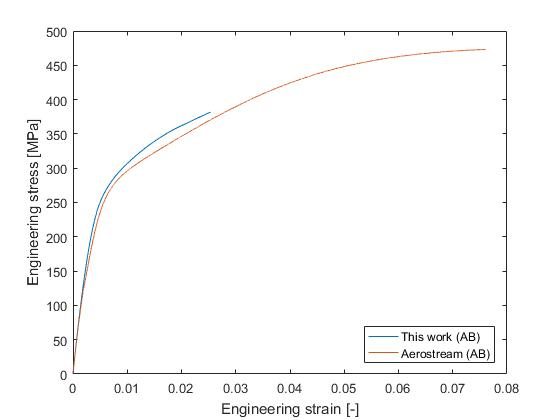
\includegraphics[scale=0.64]{Images/AerAB}}
	\decoRule
	\caption[Engineering stress-strain tensile curves for as-built specimens of this work (in average) and of \textit{Aerostream} project]{Engineering stress-strain tensile curves for as-built specimens of this work (in average) and of \textit{Aerostream} project}
	\label{fig:AerAB}
\end{figure}

The shortcomings of the manufactured samples can be attributed at least partially to the presence of residual stresses. Consequent tension residual stresses were measured in the material. The actual stress during the tensile tests was thus greater than what was measured. In addition, there is a stress concentration due to the porosities. For spherical porosities, it is given by:

$$\sigma_{loc}=K_t \cdot \sigma_{t} $$

where $\sigma_t$ is the applied stress and $K_t=\frac{3}{2}(1+\frac{2}{7-5\nu}) \simeq 2$ [-] is the stress intensity factor \parencite{Paris}. \\

The combination of the effects must have caused a shift of the actual local stress. The critical stress  $\sigma_c$ causing crack propagation was thus attained before the start of the voids coalescence, as illustrated in figure \ref{fig:RSTrac}. As a result, the apparent tensile curve was truncated, reducing slightly $\sigma_u$ and greatly $\epsilon_f$. The yield strength, however, was the same as a residual stress free sample. \\

\begin{figure}[ht]
	\centering
	\centerline{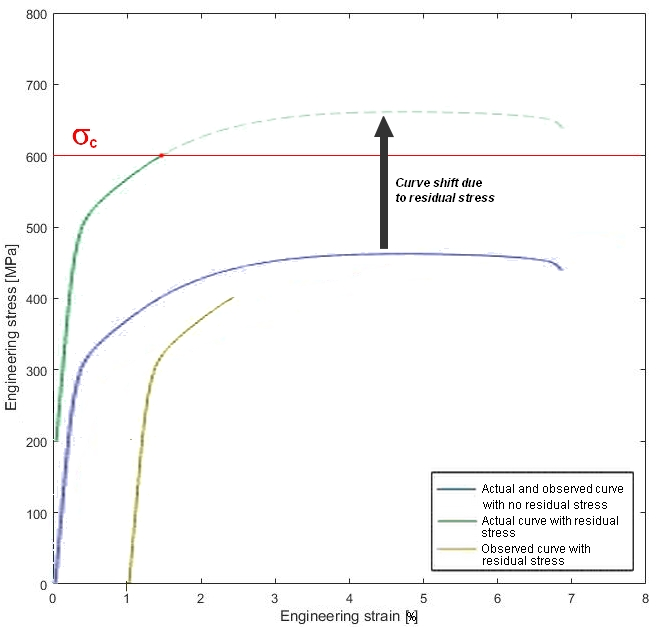
\includegraphics[scale=0.53]{Images/RSTrac}}
	\decoRule
	\caption[Illustration of the impact of residual stress on the observed tensile stress-strain curve]{Illustration of the impact of residual stress on the observed tensile stress-strain curve}
	\label{fig:RSTrac}
\end{figure}

This concurs with the data of table \ref{tab:Wang}: the heating of the plate during the manufacturing process at 160$^\circ C$, while reducing the residual stresses, increased the fracture strain by 77\%. This could explain the differences with the better properties found in literature: as all the sources that obtained both high $\sigma_u$ and $\epsilon_f$ did not specify the used process conditions, it is conceivable that they all used plate heating. \\

A consequent increase of ductility was observed for samples heat treated at 250$\sigma$ and higher temperatures. This is due to the softening of the material induced by the microstructure modifications (see section \ref{DMMM}). It could also be due to stress relief (SR). However, SR is not necessary to explain the results: the lowered maximal stress due to the softening could simply have been insufficient to reach the critical value $\sigma_c$ impeding the ductile damage mechanism. The curves can thus not enable to certify if there was stress relief or not. Nevertheless, the heat treatment at 250$^\circ C$ permitted to have a good trade-off for the tensile properties: there was an increase of 250\% of $\epsilon_f$ for decreases of only 12\% and 11\% of $\sigma_y$ and $\sigma_u$ respectively. This is quiet different from what Mertens et al. observed for the same treatment (80\% increase for $\epsilon_f$ and decreases of 10\% and 2\% for $\sigma_y$ and $\sigma_u$) \parencite{Mertens15}.\\

An increase of ultimate tensile strength was observed for the specimens that underwent a heat treatment at 150$^\circ$C. This is seemingly due to artificial ageing: precipitated $Mg_2Si$ particles constrain the dislocations displacement through the Orowan bowing phenomena as shown in figure \ref{fig:Oro}, which induces hardening \parencite{Ghosh}. Artificial ageing can take place at 160$^\circ$C (see section \ref{SOTAPT}), it thus do not seem far-fetched that it could happen ten degrees below. Sample heated at 200$^\circ C$ demonstrated properties similar to the as-built ones. This is probably due to the compensation of the age-hardening effect with the microstructure softening.\\

\begin{figure}[ht]
	\centering
	\centerline{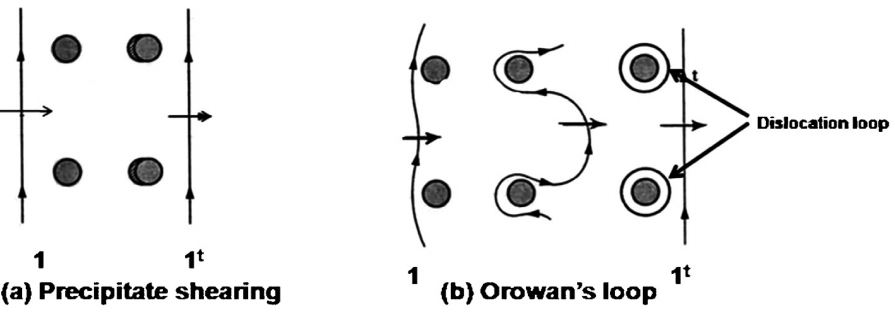
\includegraphics[scale=0.45]{Images/Orowan}}
	\decoRule
	\caption[Schematic representation of dislocation/precipitate interaction under different tempering condition (a) underaged, (b) peak aged]{Schematic representation of dislocation/precipitate interaction under different tempering condition (a) underaged, (b) peak aged (from Ghosh et al., 2015 \parencite{Ghosh})}
	\label{fig:Oro}
\end{figure}

A noteworthy parallel can be made between the Vickers hardness and the ultimate tensile strength for AB and heat treated samples. The two are connected via a quasi-linear relationship as shown in table \ref{tab:HVUTS} and figure \ref{fig:HVUTS}. A good empirical approximation can thus be obtained with $\sigma_u \simeq 2.88 H_v$. Data was taken from sections \ref{RCABS} and \ref{RCHTS}.

\begin{center}
	\begin{table}[ht]
		\centerline{\begin{tabular}{|c|c|c|c|}
				\hline
				HT & $H_v$ [HV] & $\sigma_u$ [MPa] & $\frac{H_v}{\sigma_u}$ $[\frac{HV}{MPa}]$ \\
				\hline
				AB & 136  & 381.7&2.81\\
				150$^\circ$ &151.0 & 441.7 & 2.93\\
				200$^\circ$  &133.6& 382.0 & 2.86\\
				250$^\circ$  &118.6&340.9 & 2.87\\
				300$^\circ$  &86.7& 252.9 & 2.92\\
				\hline
		\end{tabular}}
		\caption[Relationship between Vickers hardness and ultimate tensile strength]{Relationship between Vickers hardness and ultimate tensile strength}
		\label{tab:HVUTS}
	\end{table}
\end{center}

\begin{figure}[ht]
	\centering
	\centerline{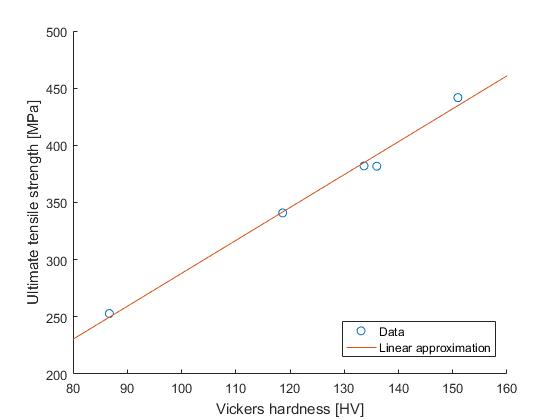
\includegraphics[scale=0.64]{Images/HVUTS}}
	\decoRule
	\caption[Average ultimate tensile strength for each heat treatment as a function of the Vickers hardness]{Average ultimate tensile strength for each heat treatment as a function of the Vickers hardness}
	\label{fig:HVUTS}
\end{figure}

\section{Microstructure}
\label{DMMM}

%[Mécanisme d'endommagement: deux populations de porosités? A confirmer/ infirmer avec les articles envoyés par AS]
%[Taille des cupules= ordre de grandeur des éléments de la microstructure?] 


%[Mécanisme d'endommagement: deux populations de porosités? A confirmer/ infirmer avec les articles envoyés par AS]

%[Taille des cupules= ordre de grandeur des éléments de la microstructure?] 
%[Mécanisme d'endommagement: deux populations de porosités? A confirmer/ infirmer avec les articles envoyés par AS]
%[Taille des cupules= ordre de grandeur des éléments de la microstructure?] 


%[Modèle pour la sphéroisisation: rien dans la literature pour notre microstructure (? j'ai rien trouvé en faisant une petite recherche)]
%[Trajet de fissure "accidenté"? Déviation par les défauts?]

Evolution of microstructure with post-treatments follows the expected spheroidization process. Optimisation of the final part microstructure - and thus mechanical properties - can however still be refined. A more accurate control of the parameters to ensure reproducibility could be needed. Further exploration of other sets of parameters, such as high temperature annealing with short holding time, could improve productivity without sacrificing quality of the part.\\

Similarity in the size of dimples on fractographs and microstructural cells is coherent with other results available in the literature. Dimple ridges could correspond to the ductile Al cells undergoing necking just before final failure.\\

\subsection{Fractography}

Step-like structures with width length similar to the hatch space were observed. It would suggest that failure takes place at the boundary between melt pools, where the microstructure is coarser, as discussed by Aboulkhair et al. \parencite{Rosenthal17}.\\

Abundance of defects such as lack of fusion and porosities indicates that tensile failure is dictated by the presence of preferential sites for crack initiation. They are one cause for the low ductility of SLM alloys but not the only one. Annealing had no observable impact on these defects.\\

%[Taille des cupules= ordre de grandeur des éléments de la microstructure?] 

%[Modèle pour la sphéroisisation: rien dans la literature pour notre microstructure (? j'ai rien trouvé en faisant une petite recherche)]
%[Trajet de fissure "accidenté"? Déviation par les défauts?]

Evolution of microstructure with post-treatments follows the expected spheroidization process. Optimisation of the final part microstructure - and thus mechanical properties - can however still be refined. A more accurate control of the parameters to ensure reproducibility could be needed. Further exploration of other sets of parameters, such as high temperature annealing with short holding time, could improve productivity without sacrificing quality of the part.\\

Similarity in the size of dimples on fractographs and microstructural cells is coherent with other results available in the literature. Dimple ridges could correspond to the ductile Al cells undergoing necking just before final failure.\\

%\subsection{Fractography}

%Abundance of defects such as lack of fusion and porosities indicates that tensile failure is dictated by the presence of preferential sites for crack initiation. They are one the cause for the low ductility of SLM alloys but not the only one. Annealing had no observable impact on these defects.

%Residual stress à discuter dans mechanical properties ok?
%\section{Residual stresses}

%[XRD: pièce as-built a un plus petit spread que ceux avec TT à basse T, p-e parce que cube coupé en 2 => relaxation des contraintes après fab?]

%While the usual stress-relief treatment for aluminium alloys -to hours holding at 300$^\circ$ C- does indeed relieve stresses inside the specimen, it also triggers significantly the diffusion of alloying elements, altering the material microstructure.



\label{D-MP}

\section{Residual stresses}
Residual stresses measured with the hole method for an as-built sample were inferior to the ones of a specimen treated at 300$^\circ C$. Other samples were sent for analysis, but the results were not received when this work was submitted due to logistical issues: the specimens were analysed in Malta, causing considerable transport time.\\

%X-ray diffraction method measurements suggested that the as-built sample had a similar amount of residual or less residual stresses compared to the heat treated samples. For heat treated samples, a diminution of residual stresses was measured as a a function of temperature. However, this trend could be insignificant as the measurements were far from was obtained in literature for stress-free samples. 

According to Vashista et al. (2012) \cite{Vashista12}, direct mathematical relation between the full width at half-maximum (FWHM) and residual stresses is difficult to obtain. This is due to the tendency of FWHM to increase with plastic deformation and grain refinement. They however observed experimentally a non-linear increase of FWHM with residual stresses.\\

We indeed observe a decrease of FWHM with the temperature of the heat treatment. It could mean that the heat treatment relieves stresses as intended. Only the as-built sample seems to defy this logic and present a FWHM lower than some heat-treated samples. However this could be explained by the geometrical difference of the as-built. While the heat-treated samples used for XRD are complete 5 x 5 x 5 [mm$^3$] cubes, the as-built is 1 x 1 x 1 [cm$^3$] cube cut in half. The higher volume explains the higher peak, and the cut may have allow a part of the residual stresses to relax by deforming the part, and thus causing the narrowing of the peak.\\


Nonetheless, the sample heat-treated at 300$^\circ$C for 2 hours remains far from stress-free according to the results from Lam et al. (2015) \cite{Lam15}. They obtained for the same peak a FWHM of 0.361, which is much smaller than everything we managed to obtain. However, as discussed above, other parameters could play a role in this difference.\\

Results obtained via the hole-drilling method appears counter-intuitive. As-built SLM samples are known for their unwanted high residual stresses, which is one the reasons for the development of many post-processes aiming at reducing them. The very low value of residual stresses in the as-built sample across the entire hole depth is thus unexpected. On the other hand, the heat treated sample present residual stresses more adequate with literature. They should however be lower than in the as-built.\\

A part of the answer could lie in the machining applied to the two parts. Indeed, installation of gauges for the strain measurements during the drilling of the hole requires a certain level of surface smoothness. The intrinsic bad surface finish of the SLM process imposed the use of a post-process to reduce rugosity. The parts were milled with cutters adapted to hard steels. The inadequacy of the tools used have probably induced compressive residual stresses near the surface. This phenomenon has probably affected the stress distribution inside the parts, but is not able on its own to explain the state of the as-built sample. Additional residual stress measurements on a larger series of samples with the same post-treatment could help to understand the causes of this phenomenon.\\


%\section{Mechanical testing}
